\section{Evaluation}
\label{sec:via:eval}

In this section, we show that \hybrid can significantly improve performance on network metrics.
Specifically, we show that:
\begin{packeditemize}
\item \hybrid achieves substantial improvement on all network metrics --- $20\%-58\%$ reduction on median (compared to the oracle's $30\%$-$60\%$; Section~\ref{sec:via:potential}) and  %\cameraremove{$37\%-78\%$}\camera{$20\%-57\%$} on $90^\text{th}$ percentile and 
$35\%-60\%$ on $99^\text{th}$ percentile. \hybrid reduces PNR by $39\%-45\%$ for the individual metrics (compared to the oracle's $53\%$ in Figure~\ref{subfig:pnr}), and by $23\%$ when PNR is computed on an "at least one bad" metric (compared to the oracle's $30\%$).
%\item Inter-domain calls benefit more from \hybrid than intra-domain calls, and the improvement differs a lot across ASes.
\item \hybrid achieves close-to-optimal performance under budget constraints by selectively relaying calls that have higher potential benefit (Section~\ref{subsec:practical-budget}).%, we see even higher improvement within the same budget. %vnp{how would budgets be applied without 4.7?}
\item {\hybrid}'s improvement increases as relay decisions are made at finer spatial granularities and more dynamically. However, we start to see diminishing gains at granularities finer than AS-pair and daily.
%\item Using ``transport'' relay (going through the backbone) have more benefit than only using ``bouncing'' relays (not going though the backbone).
\end{packeditemize}


\subsection{Methodology}
\label{subsec:eval-method}

We perform data-driven simulations based on $430$ million \skype calls (Section~\ref{subsec:dataset}). The calls are replayed in the same chronological order as in the trace thereby allowing \hybrid to gain knowledge as it goes along (using newer call measurements). We assume that when a call is assigned to certain relay option, its performance would be the same as that of a call which is randomly sampled from the set of calls between the same AS pair through the same relay option in the same $24$-hour window. Tomography-based performance prediction is made based on call performance in the last 24-hour window. For statistical confidence, in each 24-hour window, we focus on AS pairs where there are at least $10$ calls on at least $5$ relay options \footnote{Otherwise, selecting relays from a handful of candidates would be trivial. $32$ million calls  remain after these filters.}. Also, the relaying options considered for a call are only those with at least $10$ call samples. %We acknowledge this methodology makes the same simplifying assumptions as the oracle (\xref{subsec:potential-overall}). 
To quantify the confidence in the results, we also add error bars (of standard error of mean) to the graphs. Note that even with the aggregation, we used {\em distribution} (e.g., mean, percentiles) of the metrics and not per-call values for evaluation.
%We acknowledge that there are two caveats in using this methodology: 
%(1) It will give unbiased evaluation only if the relay option of each call is randomly decided (not necessarily uniformly). However, it is not desirable for service providers to let valuable users to use arbitrary relays.
%(2) Given limited number of samples on each relay option, there could be selection bias, which may make the performance of the best relay option tend to be optimistic.\vnp{unclear}

This section shows how much \hybrid can reduce PNRs (fraction of calls having poor performance on the individual network metrics or on the "at least one bad" metric), compared with the oracle approach and a strawman, such as using the \direct paths for all calls ("\direct strategy").

%\jc{remind people what PNR is}


\begin{figure}[t!]
\captionsetup[subfigure]{justification=centering,farskip=-1pt,captionskip=-1pt}
\centering
%\hspace{-0.5cm}
\subfloat[\hybrid, strawmen, oracle vs. default]
{
        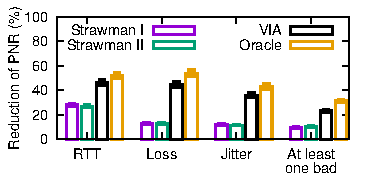
\includegraphics[width=0.5\textwidth]{figures/Via-Eval-Bar-MinChoices-5-Improvement-PNR.pdf}
        \label{subfig:eval-pnr}
}%\hspace{-0.5cm}
\subfloat[\hybrid improvement on percentiles]
{
        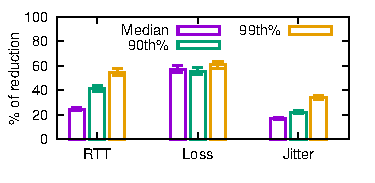
\includegraphics[width=0.5\textwidth]{figures/Via-Eval-Bar-MinChoices-5-Improvement-Percentile.pdf}
        \label{subfig:eval-perc}
}
%\vspace{-0.1cm}
%\hspace{-0.5cm}
\caption{Improvement of \hybrid. PNR on individual metrics improve by $39\%-45\%$ and on the "at least one bad" metric by $23\%$.}
\label{fig:eval-overall}
\end{figure}

\subsection{Improvement of VIA}
\label{subsec:eval-overall}

%\myparatight{Improvement on percentiles}
%Figure~\ref{fig:eval-overall} compares the performance distribution under different relay selection strategies, including ``\direct'' (always using the \direct paths), \hybrid, and the oracle logic (introduced in \Section\ref{sec:potential}). We also compare \hybrid with strawman solutions of predictive and exploratory strategies (discussed in \Section\ref{subsec:hard})\jc{names of strawmen should be changed accordingly when section 4 is done}. 
%From the figures, we can see that across all three performance metrics, \hybrid achieves close-to-oracle performance and significantly outperforms direct paths and strawmen, especially on the high tails. 
%There is \fillme\% to \fillme\% improvement at $90^{\textrm{th}}$\%ile, and \fillme\% to \fillme\% improvement at $99^{\textrm{th}}$\%ile.
%At the same time, we see that the strawman solutions have few improvements, which qualitatively confirms inefficiency of basic predictive strategies or exploratory strategies (\Section\ref{subsec:hard}).


\mypara{PNR reduction}
Figure~\ref{subfig:eval-pnr} shows the PNR reduction of \hybrid over \direct strategy (always using \direct paths), and compares it with the PNR reduction of {pure} prediction-based {selection, based just on history} (Strawman I), {pure} exploration-based selection {without any pruning of the options up front}  (Strawman II), and oracle. 
Across all three performance metrics, we see that \hybrid achieves close-to-oracle performance and significantly outperforms both the default strategy and the two strawman approaches. 
%\sout{At the same time, we see that} 
The strawman approaches yield much less improvement, which confirms the inefficiency of the {pure} predictive and {pure} exploratory strategies (Section~\ref{subsec:strawmen}).

\mypara{Improvement on percentiles} 
Figure~\ref{subfig:eval-perc} shows the improvement over \direct strategy on different percentiles.  
We first calculate the percentiles of performance of each strategy and calculate the improvement between these percentiles (which avoids the bias of calculating improvement on each call).
%The improvement on each percentile is calculated based on the percentile of extrapolated performance of all calls under different strategies (e.g., $90^{\textrm{th}}\%$ of RTT under \hybrid vs. $90^{\textrm{th}}\%$ of RTT under \direct). \vnp{unclear}  
We see that \hybrid has improved performance on both median (by $20\%-58\%$) and {the extreme} tail (by $20\%-57\%$ on $90^\text{th}$ percentile), which shows \hybrid is able to improve the performance of a wide spectrum of calls. % performance.
%\cameraremove{\myparatight{Component-wise contribution:}}

\mypara{Transit vs. bouncing relay} 
%As argued in \Section\ref{??}, an advantage of managed overlays compared to traditional overlays is that a call can avoid WAN routing by going through the backbone of the managed overlay. We define this as ``transport'' relaying, as opposed to ``bouncing'' relaying, where only one relay is used.
Finally, we find that also using transit relaying (i.e., using inter-DC connection between the {ingress and egress relays} as part of the path) usually results in higher improvement on PNR than only using bouncing relays (i.e., using one relay node to bounce off traffic). On AS pairs which have used both bouncing and transit relays, we see $50\%$ {lower} PNR when both transit and bouncing relays are available than when transit relays are excluded.
We also find that \hybrid sends about $54\%$ calls to bouncing relays, $38\%$ to transit relays, $8\%$ to \direct paths, with a marginal difference {in the distribution} across network metrics.

%\begin{figure}[t!]
%\captionsetup[subfigure]{justification=centering,farskip=-1pt,captionskip=-1pt}
%\centering
%%\hspace{-0.5cm}
%\subfloat[Prediction accuracy of tomography.]
%{
%        \includegraphics[width=0.35\textwidth]{new-figs/Tomography-error-CDF.pdf}
%        \label{subfig:eval-component-tomography}
%}\\%\hspace{-0.5cm}
%\subfloat[Various guided-exploration strategies.]
%{
%        \includegraphics[width=0.35\textwidth]{new-figs/Eval-Bar-MinChoices-5-VIA-ComponentWise-PNR.pdf}
%        \label{subfig:eval-component-ucb}
%}\vspace{-0.1cm}
%%\hspace{-0.5cm}
%\tightcaption{Component-wise analysis of \hybrid.}
%\label{fig:}
%\end{figure}

\mypara{International vs. domestic} Figure~\ref{fig:eval-inter-intra} compares PNR of international and domestic calls under strategies of \direct, \hybrid and oracle.%~\footnote{Bars in Figure~\ref{fig:eval-inter-intra} representing the \direct strategy are slightly different from those in Figure~\ref{subfig:opportunity-international}, because Figure~\ref{fig:eval-inter-intra} focuses on only calls between AS pairs where there are enough calls and have used enough relay options (\xref{subsec:eval-method})}.
We see significant improvement of \hybrid on both international and domestic calls, while international calls have a slightly higher magnitude of improvement than domestic calls. 
%We also have similar observation with respect to international calls and domestic ones. 
This can be explained by the fact that relaying has limited benefits when the bottleneck is the last-mile ISP or the last-hop connection.

%\begin{figure}[t!]
%\centering
%\hspace{-0.5cm}
%\subfloat[Inter-domain]
%{
%        \includegraphics[width=0.25\textwidth]{new-figs/Eval-Bar-Interdomain-MinChoices-5.pdf}
%        \label{subfig:}
%}\hspace{-0.5cm}
%\subfloat[Intra-domain]
%{
%        \includegraphics[width=0.25\textwidth]{new-figs/Eval-Bar-Intradomain-MinChoices-5.pdf}
%        \label{subfig:}
%}\hspace{-0.5cm}
%\tightcaption{Inter-domain vs. intra-domain. We see that \hybrid achieves improvements on both inter-domain and intra-domain calls, with a slightly higher magnitude improvement on inter-domain calls. We also have similar observation regarding international and domestic calls. \jc{Figure of international vs. domestic can be added if needed.}}
%\label{fig:eval-inter-intra}
%\end{figure}


\begin{figure}[t!]
\centering
%\hspace{-0.5cm}
\subfloat[International]
{
        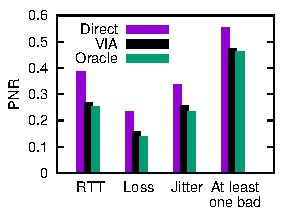
\includegraphics[width=0.45\textwidth]{figures/Via-Eval-Bar-International-MinChoices-5.pdf}
        \label{subfig:eval-international}
}%\hspace{-0.5cm}
\subfloat[Domestic]
{
        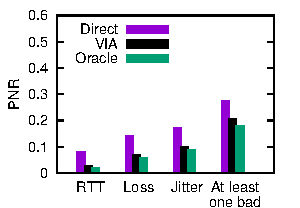
\includegraphics[width=0.45\textwidth]{figures/Via-Eval-Bar-Domestic-MinChoices-5.pdf}
        \label{subfig:eval-domestic}
}%\hspace{-0.5cm}
\caption{\hybrid improvement on international and domestic calls. 
%We see that \hybrid achieves improvements on both international and domestic calls, with a slightly higher magnitude improvement on international calls. 
We also have similar observation regarding inter-domain and intra-domain calls.}
\label{fig:eval-inter-intra}
\end{figure}


\mypara{Benefits by countries} 
Figure~\ref{fig:eval-by-name} further dissects the improvement of \hybrid by countries (with one side of the international call in that country) with worst (direct) PNR. It shows that the worst countries have a much higher (direct) PNR than the global PNR, shown by the horizontal red line, and that the performance of \hybrid is closer to the oracle than to the default for most of these countries. 


%\cameraremove{Figure~\ref{fig:eval-by-name} further dissects the improvement of \hybrid by specific countries and ASes. It shows that many countries and ASes have a much higher PNR than the global PNR (shown by the horizontal red line), and that {the performance of} \hybrid 
%{is closer to the oracle than to the default for} most of these countries and ASes. \camera{Though the figures only show the results for RTT, we also have qualitatively similar observations for the other metrics.}
%
%{That said, }there is also a substantial {disparity in the performance} improvement due to \hybrid for different countries and ASes. 
%Such difference can be explained by how relay nodes are deployed today. For instance, inter-domain calls from AS4766 and AS27947 both suffer from high RTT, but \hybrid is able to improve performance for AS4766 much more {significantly} than for AS27947, because AS4766 has direct peering connection with some relay nodes unlike AS27947.}

\begin{figure}[t!]
\centering
\subfloat[PNR of RTT]
{
        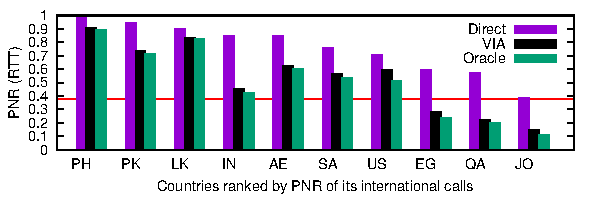
\includegraphics[width=0.75\textwidth]{figures/Via-Eval-Bar-InternationalByCountrySource-MinChoices-5-rRTT.pdf}
        \label{subfig:by-country}
}
%\vspace{-0.4cm}
\\
\subfloat[\small{PNR of loss rate}]
{
        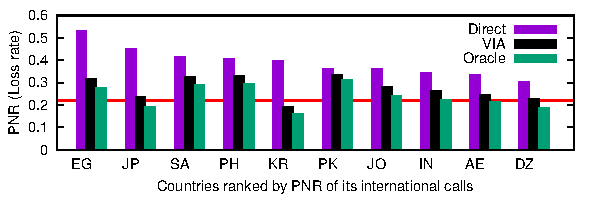
\includegraphics[width=0.75\textwidth]{figures/Via-Eval-Bar-InternationalByCountrySource-MinChoices-5-rLOSS.pdf}
        \label{subfig:by-country}
}
%\vspace{-0.4cm}
\\
\subfloat[PNR of jitter]
{
        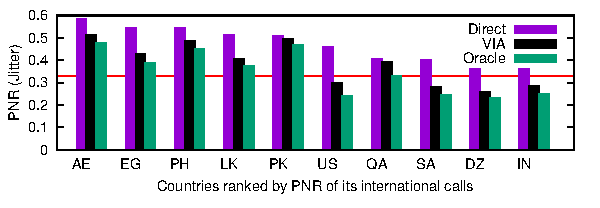
\includegraphics[width=0.75\textwidth]{figures/Via-Eval-Bar-InternationalByCountrySource-MinChoices-5-rJITTER.pdf}
        \label{subfig:by-country}
}
%\vspace{-0.2cm}
%\\
%\subfloat[Inter-domain calls grouped by AS of one side]
%{
%        \includegraphics[width=0.45\textwidth]{new-figs/Eval-Bar-InterdomainByAsnSource-MinChoices-5-rRTT.pdf}
%        \label{subfig:by-asn}
%}
%\tightcaption{Dissecting \hybrid improvement on PNR of RTT by country and AS of one side. There is a substantial diversity on \hybrid improvement across different countries and ASes. }
\caption{Dissecting \hybrid improvement on PNR by country of one side. There is a substantial diversity on \hybrid improvement across different countries. }
\label{fig:eval-by-name}
\end{figure}





%\begin{figure}[t!]
%\centering
%\subfloat[Interdomain calls grouped by source ASes]
%{
%        \includegraphics[width=0.5\textwidth]{new-figs/Eval-Bar-InterdomainByAsnSource-MinChoices-5-rRTT.pdf}
%        \label{subfig:}
%}
%\subfloat[Intradomain calls of different ASes]
%{
%        \includegraphics[width=0.5\textwidth]{new-figs/Eval-Bar-InterdomainByAsnSource-MinChoices-5-rJITTER.pdf}
%        \label{subfig:}
%}
%\tightcaption{Partitioning calls into finer-grained levels. We see a substantial diversity of performance gains between interdomain (or intradomain) calls of different ASes. }
%\label{fig:eval-spatial-partition}
%\end{figure}

\subsection{VIA's Design Choices}
\label{subsec:design}

\mypara{Prediction accuracy of relay-based tomography} 
As a first step, \hybrid uses relay-based tomography (Section~\ref{subsec:practical-prediction}) to predict the performance each \option.
We evaluated the accuracy of tomography-based predictions on the different metrics and found that on $71\%$ of calls, the predicted performance is within $20\%$ from the actual performance. However, for $14\%$ of the calls, the error can be $\geq 50\%$. This non-negligible prediction error explains the poor performance of Strawman I (pure prediction-based) that we have seen in Figure~\ref{subfig:eval-pnr}, and also motivates real-time exploration.





\mypara{Benefits of prediction-guided exploration} 
As discussed in Section~\ref{sec:via:design}, \hybrid is not a simple combination of prediction and exploration approach. 
First, instead of picking a fixed number top candidates, \hybrid pick top candidates by taking variance of prediction into account. 
Second, instead of using the original UCB1 algorithm, which assumes a normal distribution of rewards, we adopt a different way to normalize values to cope with performance outliers.
Figure~\ref{fig:eval-component-ucb} quantifies the incremental contribution of both modifications on PNR of the three metrics.
It shows that each modification makes a significant contribution to \hybrid's improvement. With the ``at least one bad'' metric, picking top $k$ and using the normalized reward reduces PNR by $24\%$ compared to $15\%$ with just the top $2$ (loss rate PNR by $44\%$ compared to $26\%$).
%the improvement of PNR from $26\%$ to $30\%$ ($15\%$ to $17\%$), and using our normalized reward, instead of standard UCB1, further raises the improvement of PNR to $44\%$ (to $23\%$).




%\subsection{Budget constraints}
%\label{subsec:eval-budget}

\subsection{Practical Relaying Factors}
\label{subsec:eval-parameter}



\mypara{Relaying budget} Being able to use relays judiciously within a budget for relayed calls is an inherent requirement in the context of managed overlay networks such as \hybrid. 
Here, we define budget as the maximum fraction of calls being relayed. {We only impose an overall budget, not a per-relay one.}
Figure~\ref{fig:eval-budget} shows the impact of budget on PNR (of at least one bad metric) of three strategies: oracle, budget-unaware \hybrid and budget-aware \hybrid. The budget-unaware \hybrid, which selects relays based on Algorithm~\ref{alg:hybrid}, will relay calls whenever there is potential benefit of doing so, without taking into consideration the overall budget {of relaying}. Therefore, there is a risk of the budget getting used up by calls with only small benefit.
%\vnp{Is there the risk of the budget getting filled up by unimportant calls?} 
In contrast, budget-aware \hybrid (Section~\ref{subsec:practical-budget}) relays a call only when the benefit is larger than a threshold, which depends on the actual budget. That means calls with minimal benefit will not be relayed, saving resources for the calls that would benefit the most by relaying.
From Figure~\ref{fig:eval-budget}, we see that the budget-aware \hybrid (Section~\ref{subsec:practical-budget}) can use budget much more efficiently than the budget-unaware \hybrid. 
Also, budget-aware \hybrid can achieve about half of the maximum benefit (i.e., when budget is $100\%$ of calls) with a budget of $0.3$ (i.e., only relying $30\%$ of calls).%\vnp{why not just stick to percentages, e.g., 30\% instead of 0.3, just to be consistent with an earlier section?}

\begin{figure}[t!]
\centering
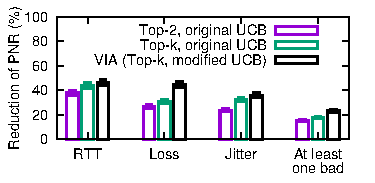
\includegraphics[width=0.6\textwidth]{figures/Via-Eval-Bar-MinChoices-5-VIA-ComponentWise-PNR.pdf}
%\vspace{-0.3cm}
\caption{Comparing guided-exploration strategies.}
\label{fig:eval-component-ucb}
\end{figure}

\begin{figure}[t!]
\centering
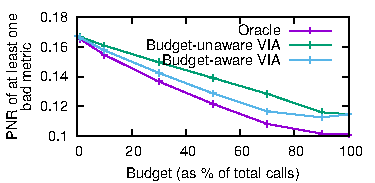
\includegraphics[width=0.5\textwidth]{figures/Via-Eval-Budget-Overall-MinChoices-5-sRTT.pdf}
\caption{Impact of budget constraint on \hybrid.}
\label{fig:eval-budget}
\end{figure}




%So far, we have evaluated \hybrid with a default set up of the managed overlay, where we have no limit on maximum number of relayed calls, and we can leverage all relays.
%Next, we show how the benefit of \hybrid can be affected by various aspect of the managed overlay, including how frequently the relay decisions are made and which relays are used.

\mypara{Relaying decision granularities}
We show performance improvement as a function of the spatial and temporal granularity at which \hybrid operates. 
First, to show the impact of spatial granularity, Figure~\ref{subfig:granularity-spatial} fixes the temporal granularity to running stage ($2$) and ($3$) of \hybrid every $24$ hours, i.e., $T=24$ hours (Figure~\ref{fig:intuition}) 
%\vnp{need to state clearly exactly which part is run every 24 hours}
 and compares the PNR if {different} relay options {could be} selected for calls in different spatial granularities. For fair comparison, the PNR are calculated based on the same set of calls.
%We show {\em PNR inflation} (dividing PNR by the PNR of making decision per AS pair every 24 hours) as a function of spatial granularities of decision making. 

We see two consistent trends. First, making decision at granularities coarser than a per AS pair results in a smaller reduction in PNR. For instance, different ISPs within a country have different peering relationships, and thus may have different optimal relay options, but such opportunities will not be exploited when making decision per country. Second, making decisions on finer granularities does not help much, though for a different reason. At finer granularities, the coverage becomes much smaller, which make \hybrid unable to predict many potential relay options.
In future work we hope to analyze a much larger data set
In Figure~\ref{subfig:granularity-temporal}, we see a similar pattern when comparing PNR of different temporal granularities, i.e., different values of $T$ (Section~\ref{subsec:Via-approach}).  
%\jc{Do we want to claim that AS pair + 24hr is a sweet point?} \ga{Need a better explanation for the second trend.} \vnp{perhaps say that in future work we hope to analyze a much larger data set}

\begin{figure*}[t!]
\centering
\hspace{-0.5cm}
\subfloat[Impact of spatial granularity]
{
        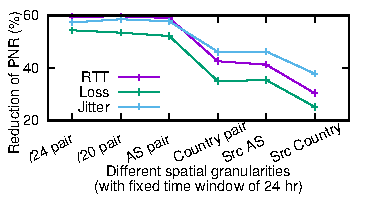
\includegraphics[width=0.5\textwidth]{figures/Via-Eval-Granularity-Spatial.pdf}
        \label{subfig:granularity-spatial}
}
\subfloat[Impact of temporal granularity]
{
        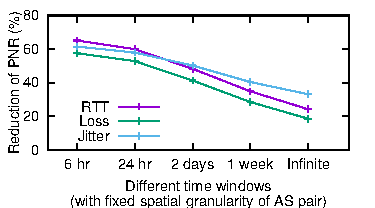
\includegraphics[width=0.5\textwidth]{figures/Via-Eval-Granularity-Temporal.pdf}
        \label{subfig:granularity-temporal}
}\\
\subfloat[Impact of relay deployment]
{
        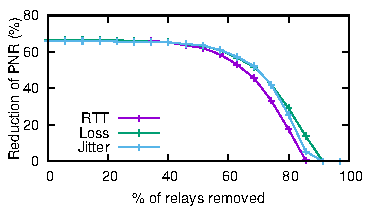
\includegraphics[width=0.5\textwidth]{figures/Via-Eval-Removing-Relays.pdf}
        \label{subfig:eval-deployment}
}
%\hspace{-0.5cm}
\caption{Sensitivity analysis of \hybrid improvement. 
Figure~\ref{subfig:granularity-spatial} and \ref{subfig:granularity-temporal} compares PNR under different control granularities. Figure~\ref{subfig:eval-deployment} shows PNR when some of the (least used) relays are excluded.}
\label{fig:eval-granularity}
\end{figure*}


\mypara{Relay usage} 
Figure~\ref{subfig:eval-deployment} shows reduction of PNR when a subset of (least used) relays is excluded. We see that the contribution of benefits from different relay nodes are highly skewed. Removing $50\%$ of the (least used) relays causes little drop in \hybrid's gains. This suggests that new relays should be deployed carefully in future. 

%\begin{figure}[t!]
%\centering
%\includegraphics[width=0.35\textwidth]{new-figs/Eval-Removing-Relays.pdf}
%\tightcaption{PNR inflation when $n$ least used relays are excluded. We see that the least used 30 relay nodes contributes a tiny fraction of benefit compared with the most used 30 relays nodes.}
%\label{fig:eval-deployment}
%\end{figure}


%Figure~\ref{fig:eval-turnturn} compares the PNR of direct paths, using only bouncing relays (and direct paths), and using all three of bouncing, transport and direct paths. For a fair comparison, we focus on the AS pairs where both bouncing relaying and transport relaying are available. To get the PNR of using only bouncing relays, we run \hybrid algorithm and set the budget of relay options that involve two relays to be zero. 
%We see that though using only bouncing relays can achieve substantial improvement over direct paths, using transport relay can further reduce PNR, especially on loss rate. \jc{We need to say something to justify the marginal additional benefit of transport -- this is really due to the fact that NGC only uses transport relaying in rare cases, which make it hard to even stitch together a transport path in anyway.}

%
%\begin{figure}[t!]
%\centering
%\includegraphics[width=0.35\textwidth]{new-figs/Eval-Bouncing-vs-turnturn.pdf}
%\tightcaption{Comparing PNR of direct paths, using only bouncing relays (and direct paths), and using all three of bouncing, transport and direct paths. We see that though using only bouncing relays can achieve substantual improvement over direct paths, using transport relay can further reduce PNR, especially on loss rate.}
%\label{fig:eval-turnturn}
%\end{figure}

\subsection{Real-World Controlled Deployment}

%The data-driven evaluation (\xref{subsec:eval-method}) we have been using so far is fundamentally limited by two factors -- (1) Since we are not in a position to change the \skype client, it is infeasible to verify how much an {\em individual} caller-callee pair can benefit from using a different relay selected by \hybrid, and (2) Since it is impractical to ask valuable clients to use arbitrary relays, we are not able to quantify the {\em full} potential of \hybrid.
%In this part, we use a controlled experiment platform to address these concerns, though at a very small scale. 
%The platform implements all the key components of \hybrid (\xref{subsec:arch}). We deploy instrumented \skype clients in five countries, and use a centralized controller to instrument the client pairs to make calls using specific \option (\direct paths, bouncing relays or transit relays). 
%After each call, the measured statics of RTT, jitter, and loss are sent back to the controller to inform further decisions.
%Essentially, the controlled experiment platform allows us to measure the performance of the same caller-callee pair on many \options (including those not tried in our dataset) at roughly the same time (e.g., within an hour) and verify the effectiveness of \hybrid (albeit at a very small scale). 

We implemented and deployed a prototype containing the relevant components of \hybrid at a small scale using modified \skype clients and using {\skype}'s production relays. The central controller of our prototype (Figure~\ref{fig:mdn-overview}), deployed on the public Microsoft Azure cloud, aggregated performance measurements from instrumented \skype clients and implemented the relay selection algorithm. The instrumented \skype clients contacted the controller to decide which of the relays of \skype, if any, to use for their calls. We deploy the instrumented client on $14$ machines across Singapore, India, USA, UK and Sri Lanka. Overall, we required minimal modifications to the \skype client.

The controller also orchestrated each client to make calls to the other clients. In total, it created around 1000 calls between $18$ caller-callee pairs. Specifically, it instructed each caller-callee pair to make (short) back-to-back calls using $9-20$ different \options, $4-5$ times each. Since our testbed is at a small scale, such back-to-back calling provides us with high density performance samples between source-destination pairs through many different relays.  We use these samples to perform a controlled experiment on {\hybrid}'s relaying heuristic with accurate ground truth. For simplicity, we omit the direct path as an option.

The results are shown in Figure~\ref{fig:real-world}, where each curve shows the CDF of ``sub-optimality'' of \hybrid's performance on each call, defined by $\frac{\text{Perf}_{\hybrid}-\text{Perf}_{\text{oracle}}}{\text{Perf}_{\text{oracle}}}$.
We found that {\hybrid}'s relaying decision is within $20\%$ of an oracle's performance for $70\%$ of the calls. Note that this is despite picking the {\em best} relay (i.e., sub-optimality of $0$) for no more than $30\%$ of the calls. When there are multiple relaying options with similar performance, temporal fluctuations may lead to not always picking the best option. But \hybrid usually picks the option that is close in performance to the best.
%\cameraremove{We find that {\hybrid}'s relaying decision is within $5\%$ of an oracle's performance for more than $95\%$ of the calls.}


\begin{figure}[t!]
\centering
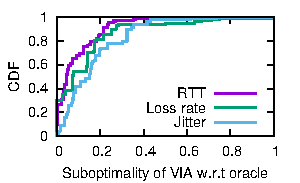
\includegraphics[width=0.45\textwidth]{figures/Via-Rajdeep-active-exp-CDF.pdf}
\caption{Deployment results. CDF, over calls, of sub-optimality (lower is better) of \hybrid's performance.}
\label{fig:real-world}
\end{figure}


%\commentout{
%\camera{
%\begin{table}[t!]
%\centering
%\begin{footnotesize}
%\begin{tabular}{ccccc}
%   Pairs    & Location & Oracle & \hybrid & Default \\ \hline\hline
%Pair A & N. America - S. Asia & 235    & 248 & 282     \\ \hline
%Pair B & N. America - S.E. Asia & 252      & 254  & 269      \\ \hline
%Pair C & S. Asia - S.E. Asia & 45   &  46 &     45
%\end{tabular}
%\end{footnotesize}
%\tightcaption{Example of real-world validation results. Each cell represents the average RTT (ms) of each strategy.}
%\label{tab:real-world}
%\end{table}
%
%\camera{To provide more detail results of the controlled experiments, Table~\ref{tab:real-world} compares the average RTT of \hybrid strategy, \direct path and oracle strategy on three specific client pairs. We pick these client pairs as they represent distinct geographical characteristics -- Pair A is between two long distance wireless clients, Pair B is between two long distance Ethernet clients, and Pair C is between (relatively) short distance clients. 
%While \hybrid achieves close-to-optimal performance, we also make two interesting observations pertaining to the nature of these client pairs.
%First, one would expect it is more likely for \hybrid to find the best \option for Pair A than for Pair B, because the performance gap between the best relay (i.e., Oracle) and \direct path of Pair A (235ms vs. 282ms) is much larger than Pair B (252ms vs. 269ms). Yet, \hybrid's performance is closer to optimal on Pair B than on Pair A, because Pair A is between two wireless clients, whose noisy performance makes it more difficult for \hybrid to identify the best decisions for Pair A than for Pair B (which is between ethernet clients).
%Second, the fact that the \direct path is the best choice for Pair C while using certain relay is the best for Pair A and B echoes one of the observations in \S\ref{sec:motivation} that long-distance calls benefit more from relaying. 
%}
%}
%
%
%%The data-driven evaluation (\xref{subsec:eval-method}) we have been using so far is unable to estimate how much an {\em individual} caller-callee pair can benefit if it were to use the relay selected by \hybrid that was not used by it in the dataset. 
%%Since for now, we are not in a position to change the \skype client, this is a fundamental limitation of using passively collected measurements.
%%In this part, we use a controlled experiment platform to address this concern, though at a very small scale. 
%%The platform implements all the key components of \hybrid (\xref{subsec:arch}). We deploy instrumented \skype clients in five countries, and use a centralized controller to instrument the client pairs to make calls using specific \option (\direct paths, bouncing relays or transit relays). 
%%After each call, the measured statics of RTT, jitter, and loss are sent back to the controller to inform further decisions.
%%
%%Essentially, the controlled experiment platform allows us to measure the performance of the same caller-callee pair on many \options at roughly the same time and verify the effectiveness of \hybrid (albeit at a very small scale).
%%Specifically, we let each pair of caller and callee to make back-to-back calls (each of 2 minutes) using 10 different \options. This provides the performance measurements of 10 \options for the same caller-callee pair at roughly the same time (i.e., within 20-minute window).
%%Then, we repeat this process for multiple rounds, to get this complete set of measurements over a period of time. Based on this dataset, we can evaluate the behavior of \hybrid more accurately.
%%
%%Table~\ref{tab:real-world} compares the average RTT of the \options selected by \hybrid with that of \direct and oracle strategies. 
%%%The relays are chosen based on geographical proximity (i.e., none of the relays is clearly worse than others in a geographical sense).
%%We choose three client pairs as each of them represents a unique scenario.
%%Pair A and Pair B are long-distance calls, while Pair C has relatively shorter distance calls. Furthermore, Pair A is between two wirelessly connected home machines, and Pair B is between two wiredly connected campus machines. Note that such case study with machine-specific information is rarely feasible in the passively measured dataset.
%%Overall, we see that \hybrid is able achieve close-to-optimal performance.
%%In addition, there are two observations pertaining to the nature of each pair. 
%%(1) The fact that the direct path is the best choice for Pair C while using certain relay is the best for Pair A and B reinforces the observation that relay has a larger benefit on long-distance calls. 
%%(2) Pair A has a larger performance gap between its best relay path and the \direct path than Pair B does, which seems to suggest \hybrid should identify the best relay of Pair A more easily. Interestingly, we see that \hybrid has more close-to-optimal performance on Pair B than on Pair A. This is because Pair A (whose end points are wireless connection) has larger performance variation than Pair B (whose end points are wiredly connected), which makes it relatively more difficult for \hybrid to identify the better decision.
%}
%We also see that despite the geographical proximity, some relay options have even worse performance than others and the \direct path, suggesting that data-driven relay selection is necessary.
%In addition, we find a substantial variation of performance even on the same caller-callee pair using the same \option within an hour (figure omitted), which reinforces that the challenge of performance variability (\xref{subsec:strawmen}) is inherent.

%\jc{Venkat, do you think the second part is necessary?}
%Second, several relay options our experiments have not been used in our dataset (either because it was not deployed or due to incrementality in the deployment). We see that these relay options in general have similarly good performance to others, and sometimes, even better. 
%This makes a case for \skype production system to deploy \hybrid to select relays over a large pool of relay choices, which would both benefit the performance and increase the budget for relayed calls (which as \xref{subsec:eval-budget} shows, has significant benefit on performance).


%\subsection{Real-world validation}
%\jc{Two messages:
%\begin{packeditemize}
%\item Validate the best relays chosen by the offline decision-making algorithm. Basically, I can provide Rajdeep with a list of best relay options from the set of relays visible to me, and we can check how close is the real performance of the relay recommended by me and that of the best relay found in Rajdeep's dataset. If the gap is too large, we can compare it with the best relay among the same set of relays (I.e., both Rajdeep and I choose relay from the set of relays visible to me).
%\item Evaluate performance of other relay options that haven't been tried (this may bring a little contradiction to section 3), and say we are deploying this system in an incremental manner, and there would larger improvement with more complete deployment.
%\end{packeditemize}}




